\chapter{Install the Firmware}\label{ch:firmware}

This chapter tells you how to load the firmware into the ClearCore. The
easiest way is from the desktop app (section~\ref{sec:fw-app}). To build the
firmware from its source, use the procedure in
section~\ref{sec:fw-build}.

\section{What You Need}

\begin{itemize}
  \item A USB cable from the computer to the ClearCore.
  \item A 24~V supply for the ClearCore. The board must not get its power
        only from USB when it writes its settings.
  \item From the app: the ClearHPGL desktop app. It carries the firmware and
        the flash tool in its \file{firmware} directory.
  \item To build from the source: a Windows computer with Microchip Studio 7
        (formerly Atmel Studio 7) and the ClearHPGL source repository. The
        build script uses the ARM compiler and the \file{make.exe} of
        Microchip Studio. The repository contains the flash tools:
        \file{tools/bossac/bossac.exe} and \file{tools/flash_clearcore.cmd},
        from Teknic.
\end{itemize}

\section{Update from the App}\label{sec:fw-app}

The desktop app carries the firmware that it was built with. It can put that
firmware on the ClearCore over USB. You do not need Microchip Studio or a
command line.

\begin{warning}
Updating restarts the board. Make sure that no job is plotting and that the
work area is clear. If the motors are enabled, the update disables them
first.
\end{warning}

\begin{procedure}{Update the firmware from the app}
\begin{enumerate}
  \item Connect the ClearCore to the computer with the USB cable.
  \item In the app, select \menu{Plotter\,>\,Update board firmware\ldots}. If
        the app is connected to the board over USB, it disconnects first.
  \item In \menu{USB port}, select the ClearCore. The window shows the
        firmware on the board and the firmware that the app carries
        (figure~\ref{fig:fwdialog}).
  \item Click \menu{Update to} (or \menu{Reinstall}) and wait. Do not
        disconnect the cable.
  \item Make sure that the window shows ``Firmware \ldots\ is running.''
  \item Click \menu{Close}. The app connects to the board again.
\end{enumerate}
\end{procedure}

\begin{figure}[htbp]
\centering
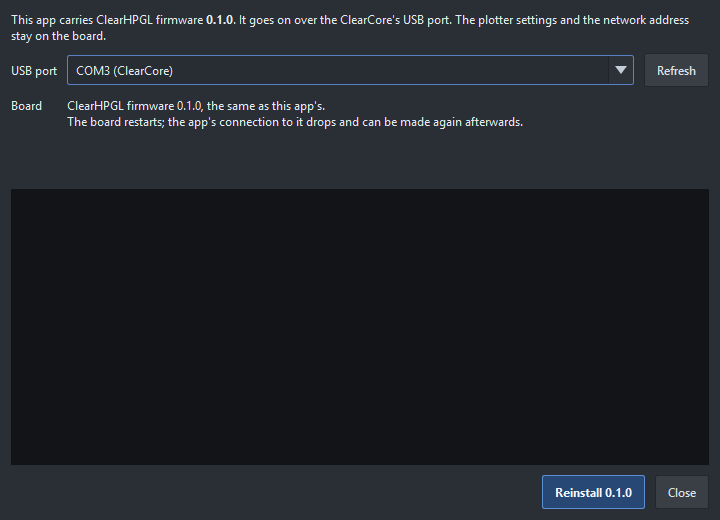
\includegraphics[width=0.8\linewidth]{firmware-dialog.png}
\caption{\menu{Update board firmware}, with the board read on COM3}\label{fig:fwdialog}
\end{figure}

The update keeps all settings of the board: the plot area, the speeds, and
the network address. They are in a part of the memory that the update does
not erase. The update does not start while a job plots.

\section{Flash Without the App}\label{sec:fw-cmd}

The installer also puts a flash tool in the \file{firmware} directory of the
app. Use it if the app cannot run.

\begin{procedure}{Flash the firmware from the Start menu}
\begin{enumerate}
  \item Connect the ClearCore to the computer with the USB cable.
  \item Close the ClearHPGL app. It can hold the USB port.
  \item Select \menu{ClearHPGL\,>\,Flash the ClearCore firmware (USB)} in the
        Start menu.
  \item Wait until the window shows \code{Success!}, then press a key.
\end{enumerate}
\end{procedure}

This also keeps the settings of the board.

\begin{note}
\notelabel If the update stops (for example, the cable is disconnected), the
board can have no firmware. Push the reset button of the ClearCore two times
quickly, so that the IO-0 to IO-5 lights move in sequence. Then click
\menu{Refresh} and update again.
\end{note}

\section{Build and Load the Firmware}\label{sec:fw-build}

\begin{warning}
Loading firmware restarts the board. Make sure that no job is plotting and
that the work area is clear before you start.
\end{warning}

\begin{procedure}{Build the firmware and load it into the ClearCore}
\begin{enumerate}
  \item Connect the ClearCore to the computer with the USB cable.
  \item Close all programs that use the USB COM port of the board: a serial
        terminal, the desktop app, or a CAD plotter driver.
  \item Open PowerShell in the root directory of the repository.
  \item Type this command and press Enter:
\begin{lstlisting}[language=console]
./Firmware/build.ps1 -Flash
\end{lstlisting}
  \item Wait. The script builds LwIP, libClearCore, and the firmware. Then it
        finds the board, puts it into its bootloader, and writes the
        firmware.
  \item Make sure that the output contains the line \code{Verify successful}.
\end{enumerate}
\end{procedure}

Without \code{-Flash}, the script only builds. The firmware files are in
\file{Firmware/ClearCoreFirmware/Release/}: \file{ClearHPGL_Firmware.bin} and
\file{ClearHPGL_Firmware.uf2}. To load a \file{.bin} file that you received
from a different person, use this command:

\begin{lstlisting}[language=console]
tools\flash_clearcore.cmd path\to\ClearHPGL_Firmware.bin
\end{lstlisting}

\begin{note}
\notelabel The flash script looks for the board on its normal USB port. Then
it waits for the bootloader port. The two ports have different COM numbers.
This is correct. If the script cannot find the board, push the reset button
of the ClearCore two times quickly to start the bootloader, then run the
script again.
\end{note}

\section{Make Sure That the Firmware Operates}

\begin{procedure}{Examine the firmware after you load it}
\begin{enumerate}
  \item Open the USB COM port of the board in a serial terminal (for example
        PuTTY). The baud rate has no effect.
  \item Type \cmd{menu} on a line by itself and press Enter. The console
        shows its list of commands.
  \item Type \cmd{version} and press Enter. Make sure that the version is the
        one that you loaded.
  \item Type \cmd{status} and press Enter. Make sure that \code{fault=none}.
  \item Type \cmd{exit} and press Enter to close the console.
\end{enumerate}
\end{procedure}

The settings stay in the board when you load new firmware. A new firmware
version that adds a setting gives it its default value.

\section{Settings of Other Firmware}

The settings of ClearHPGL have their own marker (\code{CHPG}) in the
nonvolatile memory. If the board ran ClearCoreROS or ClearAI before, and
ClearHPGL has no saved settings yet, ClearHPGL keeps the network settings of
that firmware, so the board keeps its IP address. All other settings start at
their defaults.
